\section{Destination Tickets \& Effective Resistance}

\subsection{Destination Tickets \& Winning}
Destination Tickets are rarely helpful
\begin{figure*}[!ht]
\centering
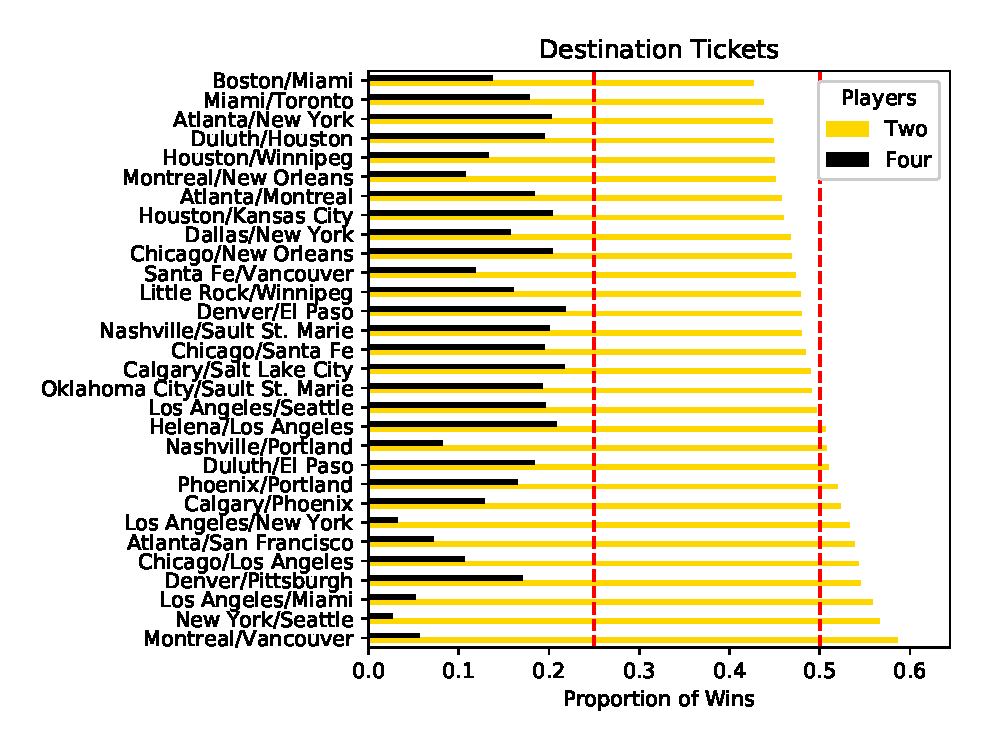
\includegraphics[scale=.8]{figures/destination_tickets}
\caption{The proportion of times that a player with a certain
Destination Ticket in their hand won.
The vertical red lines at $x=1/4$ and $x=1/2$ represent
the expected proportion of times a player with a certain Destination Ticket
would win if there was no affect. (Computed from 1000 simulations.)}
\label{fig:tickets}
\end{figure*}

\subsection{Effective Resistance}

Can effective resistance help?
\begin{figure*}[!ht]
\centering
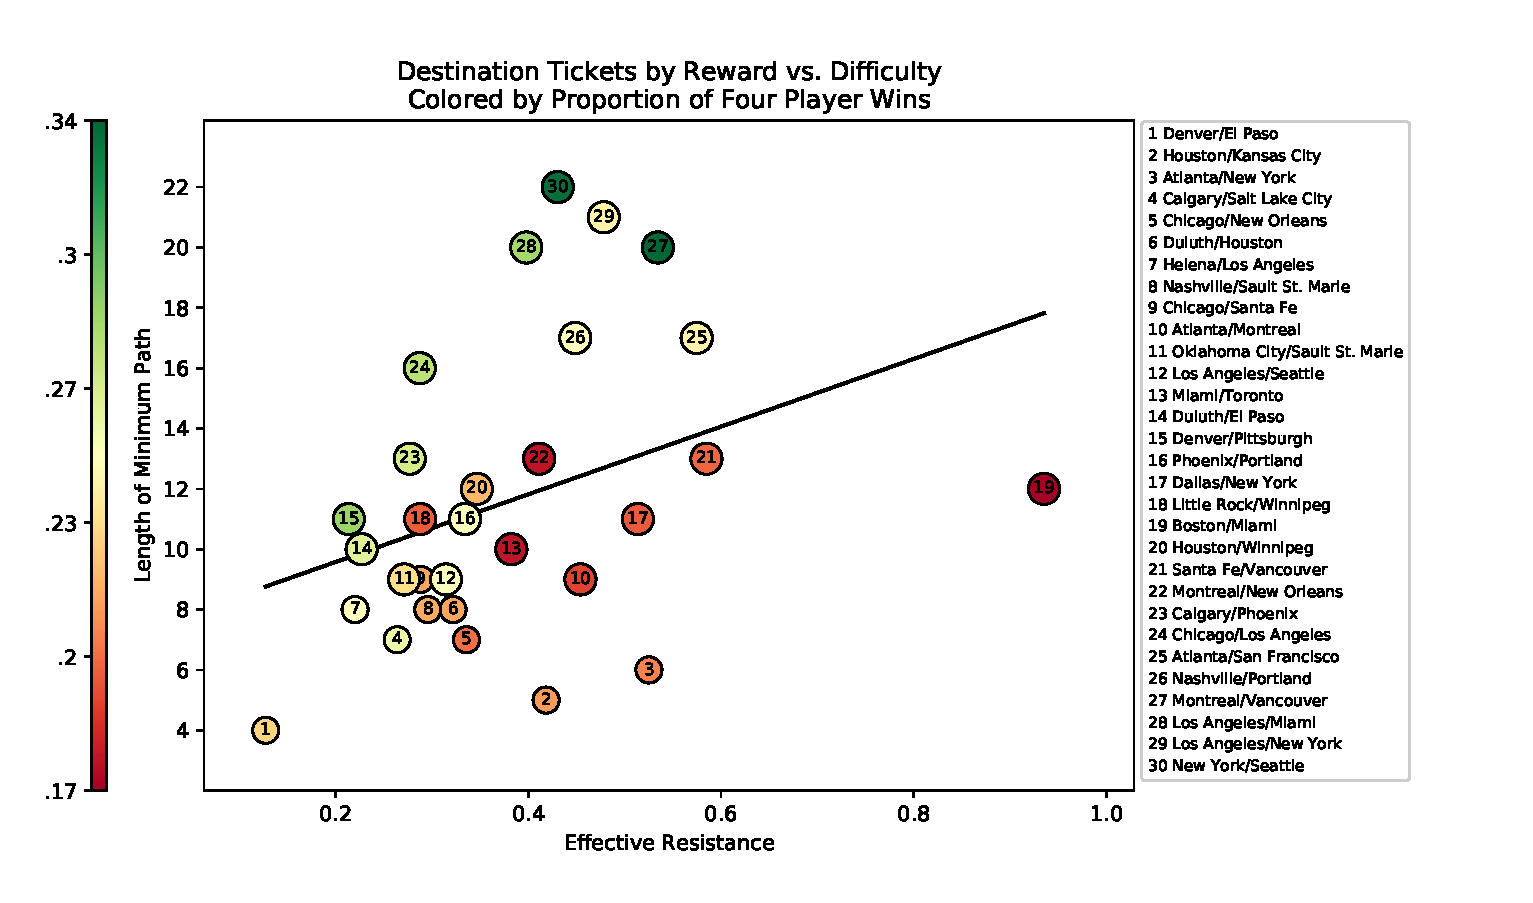
\includegraphics[scale=.8]{figures/resistance_four}
\caption{Destination Tickets by their effective
resistance and minimum path length.
The line of best fit gives an approximation of the
Destination Tickets that are better deals (above the line).
Note: the $16^{th}$ Destination Ticket Portland/Phoenix is obscured
by the $18^{th}$.}
\label{fig:resistance}
\end{figure*}

\begin{figure*}[!ht]
\centering
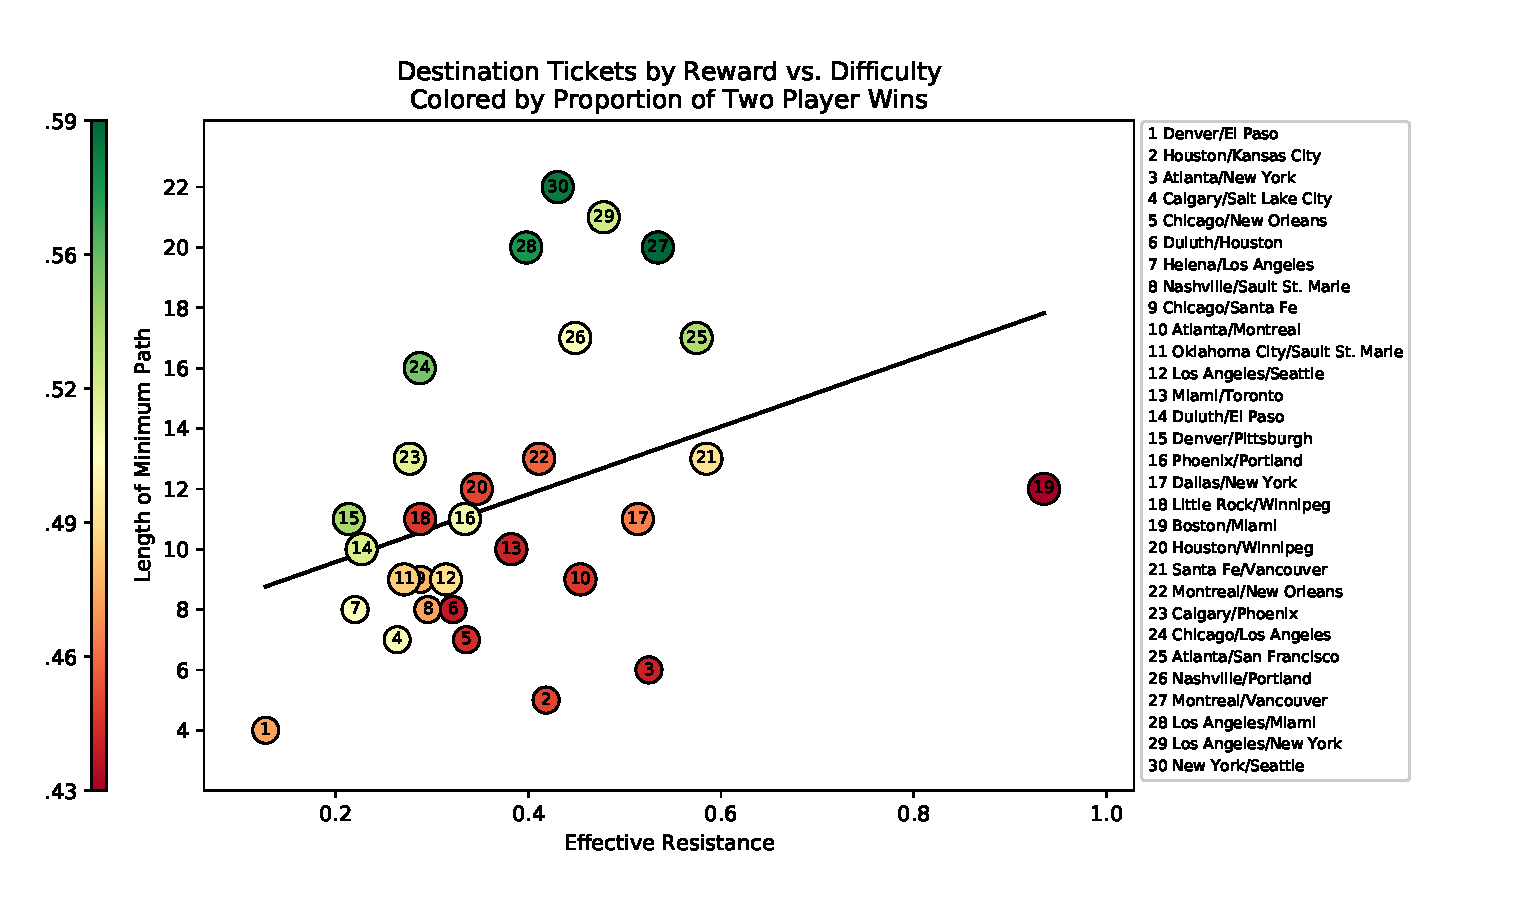
\includegraphics[scale=.8]{figures/resistance_two}
\caption{Destination Tickets by their effective
resistance and minimum path length.
The line of best fit gives an approximation of the
Destination Tickets that are better deals (above the line).
Note: the $16^{th}$ Destination Ticket Portland/Phoenix is obscured
by the $18^{th}$.}
\label{fig:resistance}
\end{figure*}
